\chapter{引言}\label{chap:introduction}

\section{背景及意义}	
\subsection{乳腺分型}
乳腺腺体类型依据美国放射学会提出的乳腺影像报告和数据系统(BI-RADS系统)分为四种类型——脂肪型乳腺、散在纤维腺体型乳腺、不均匀致密型乳腺及极度致密型乳腺,而如图\ref{fig:intro_mamtype}可以得知,不均匀致密型乳腺及极度致密型乳腺因腺体遮挡会降低对微小病变的检出率,尤其是非钙化型病变。医学研究表明,其中致密型乳腺的人群罹患乳腺癌的概率比脂肪型增加4-6倍\cite{胡从依2015数字化乳腺}。
\begin{figure}[!htbp]
    \centering
    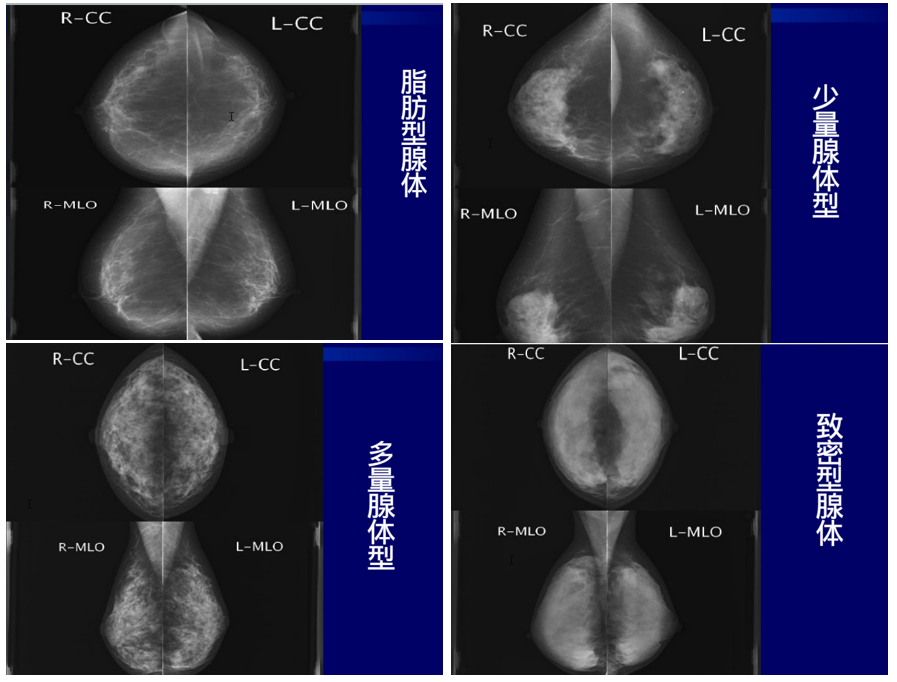
\includegraphics[width=1.0\textwidth]{intro_mamtype}
    \bicaption{乳腺钼靶分型}{Mammography target classification}
    \label{fig:intro_mamtype}
\end{figure}

乳腺钼靶问题的病灶分成肿块、钙化(如图\ref{fig:intro_calc})、结构扭曲(如图\ref{fig:intro_jiegou})、特殊征象(如图\ref{fig:intro_teshu})等多种类型。钙化分布多样,形态存在典型良性钙化,高度恶性钙化,钙化和不定性钙化等多种类型,大小一般为0.5mm到1mm之间;结构扭曲无确定的肿块可见,常见于手术后疤痕,硬化性乳腺病,浸润性导管癌等;特殊征象主要非对称性乳腺组织,局灶性非对称致密类型\cite{杨秋红2005乳腺癌的影像学诊断及进展}。

本文重点研究和考虑肿块类型数据,肿块是对乳腺不同角度拍摄都能显示的病变,其形状包括圆形、软圆型、分叶型、不规则型等,边缘存在清晰、小分叶、模糊、浸润和星芒状等情况,拥有高密度、等密度、低密度、含脂肪密度等不同密度。对于肿块病灶中常见的浸润性导管癌,其大小小于1cm(如图\ref{fig:intro_mass})\cite{31鲍润贤2002中华影像医学乳腺卷}。良恶性肿块之间区别并不明显,这需要专门研究病灶所包括的良恶性信息,进而对诊断提供帮助。
\begin{figure}[!htbp]
    \centering
    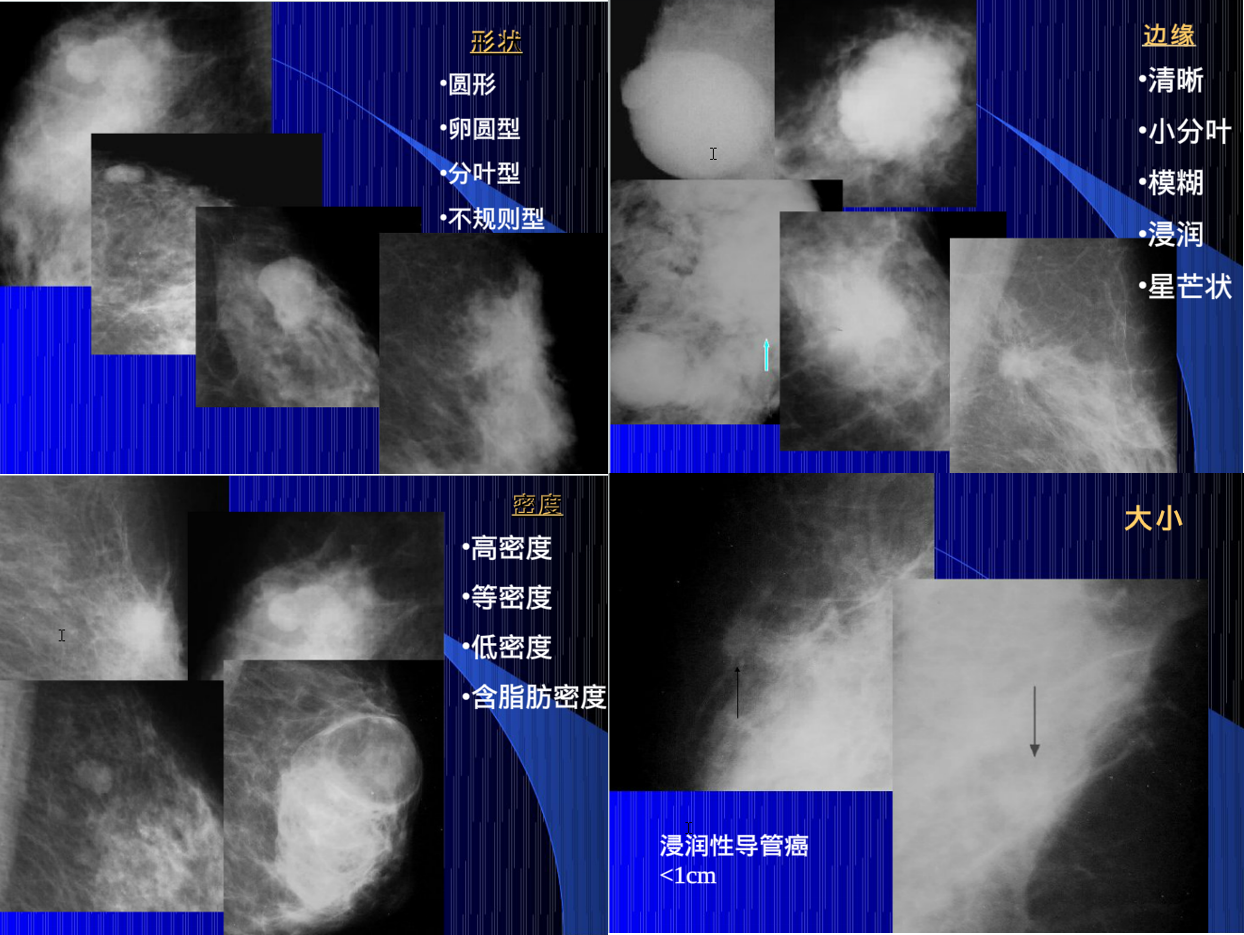
\includegraphics[width=1.0\textwidth]{intro_mass}
    \bicaption{乳腺钼靶肿块病灶特点}{Mammography's mass characteristics}
    \label{fig:intro_mass}
\end{figure}

\begin{figure}[!htbp]
    \centering
    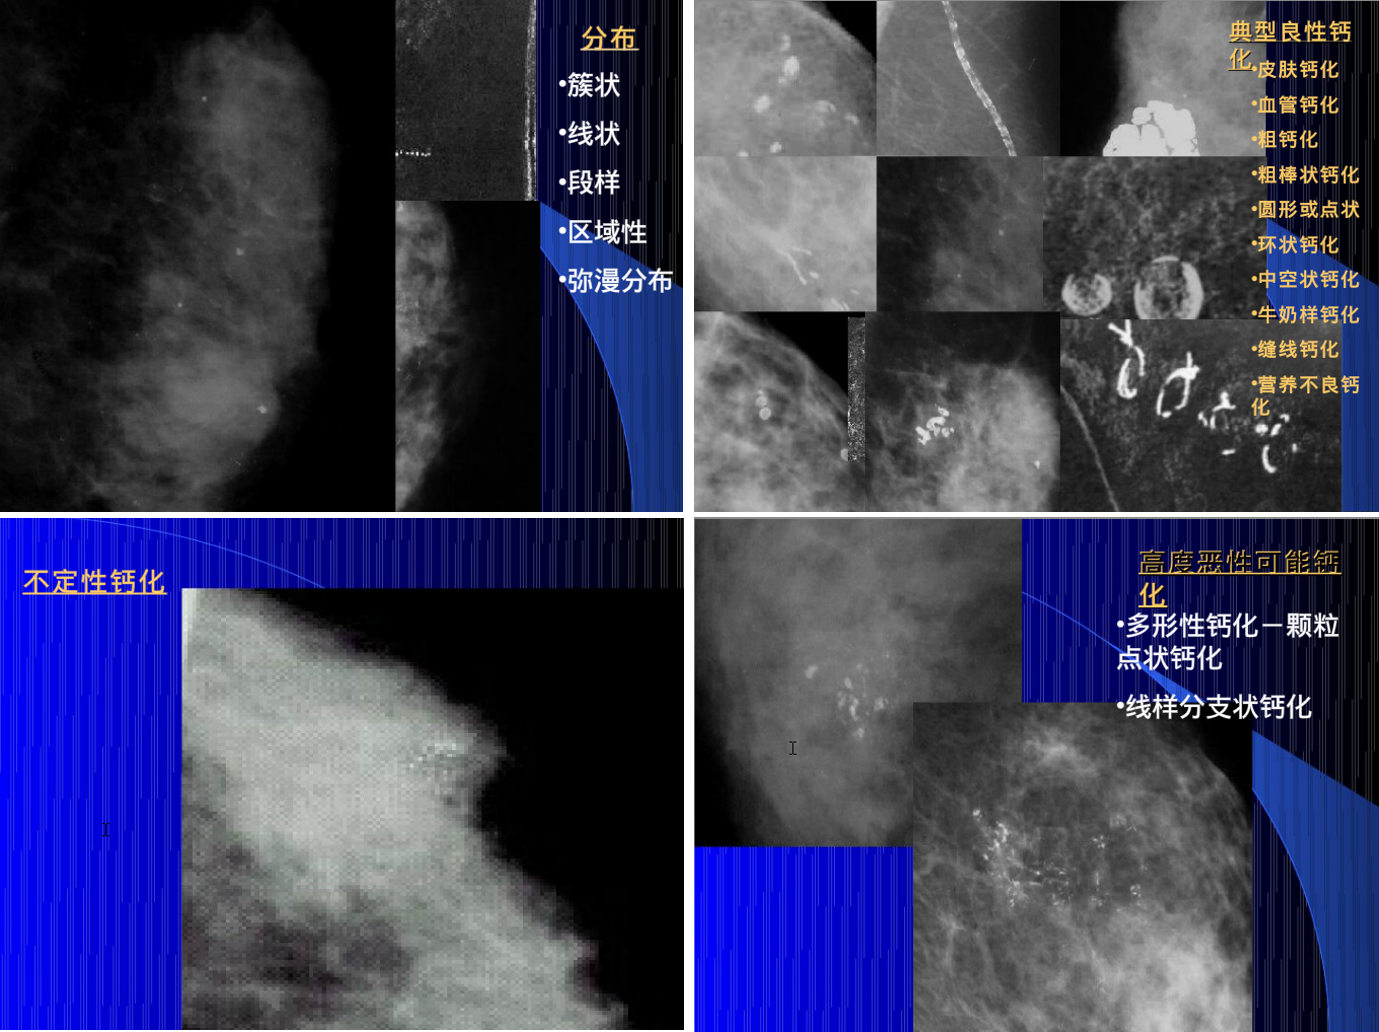
\includegraphics[width=1.0\textwidth]{intro_gaihua}
    \bicaption{乳腺钼靶钙化病灶特点}{Mammography's calc characteristics}
    \label{fig:intro_calc}
\end{figure}

\begin{figure}[!htbp]
    \centering
    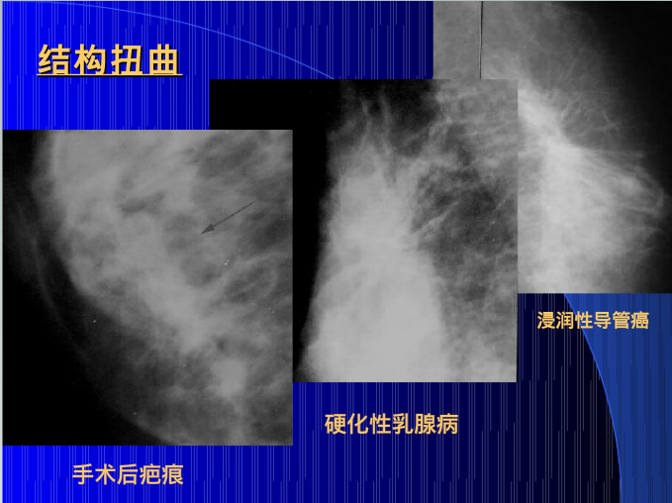
\includegraphics[width=0.6\textwidth]{intro_jiegou}
    \bicaption{乳腺钼靶结构扭曲病灶特点}{Mammography's distortion characteristics}
    \label{fig:intro_jiegou}
\end{figure}

\begin{figure}[!htbp]
    \centering
    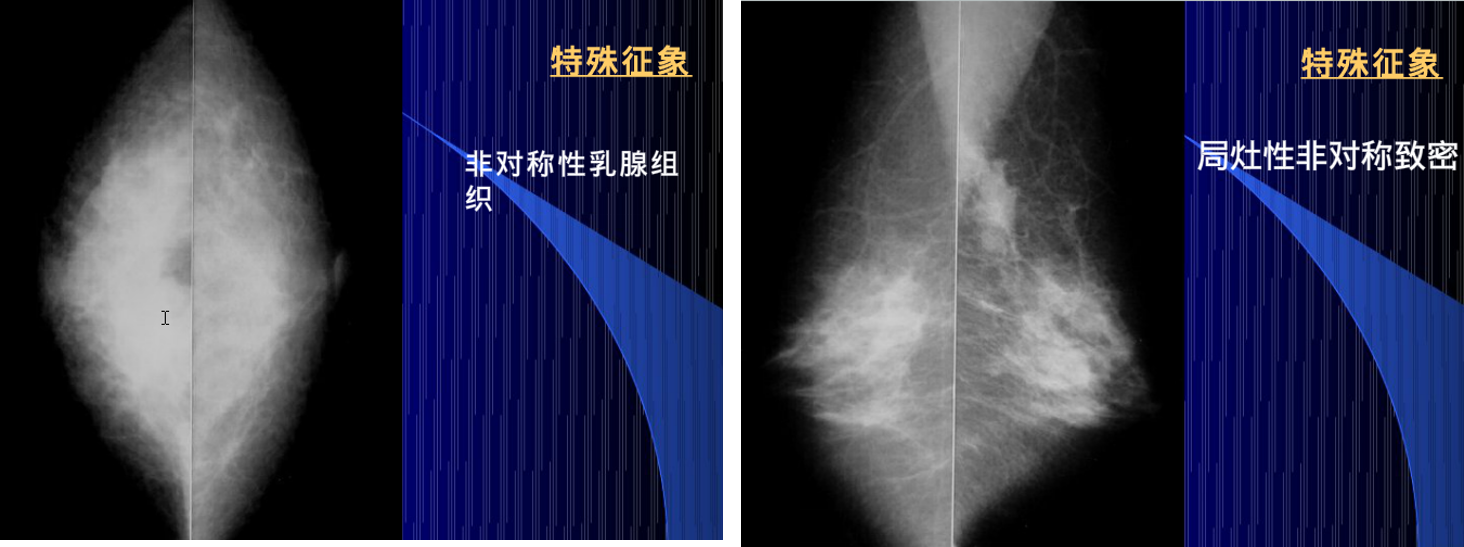
\includegraphics[width=1.0\textwidth]{intro_teshu}
    \bicaption{乳腺钼靶特征征象病灶特点}{Mammography's Characteristic signs characteristics}
    \label{fig:intro_teshu}
\end{figure}

\subsection{乳腺癌及乳腺钼靶}
乳腺癌是女性最常见恶性肿瘤之一,其发病率逐年上升。在欧美国家,乳腺癌占女性恶性肿瘤的25\%-30\%。20世纪末的统计资料表明全世界每年约有130万人诊断为乳腺癌,而有40万人死于该病。全球肿瘤流行病统计数据认为乳腺癌是中国女性最常见的癌症,年龄标化率(ASR)为每10万人21.6例。根据中国国家肿瘤登记中心的数据,乳腺癌是城市女性最常见的癌症,是农村女性第四大常见癌症。城市地区的 ASR(34.3例/10万女性)是农村地区的2倍(17.0 例 /10 万女性)\cite{1li2012analysis}。乳腺癌在城市中的发病率为女性恶性肿瘤的第二位,一些大城市已经上升至第一位,农村中为第五位。乳腺癌已经成为妇女健康的最大威胁,如表\ref{tab:basic_info_mam}所示。
\begin{table}[!htbp]
    \bicaption{我国乳腺癌基本情况}{Basic situation of breast cancer in China}
    \label{tab:basic_info_mam}
    \centering
    \footnotesize% fontsize
    \setlength{\tabcolsep}{4pt}% column separation
    \renewcommand{\arraystretch}{1.2}%row space 
    \begin{tabular}{ccccc}
        \hline
        我国乳腺癌& 2012年人数& 2012年占全球比& 至2030年增幅& 居女性恶性肿瘤排名\\
        \hline
        发病& 18.7万& 11.2\%& 29.8\%& NO.1\\
		死亡& 4.8万& 9.2\%& 47.4\%& \\
        \hline
    \end{tabular}
\end{table}

随着影像技术的快速发展,X线、超声等影像技术已逐渐成为肿瘤检出、分期及随访的重要手段,而大量的影像数据在提高疾病诊断准确性的同时也增加了疾病诊断的复杂性和对医师经验的依赖性。乳腺钼靶,全称乳腺钼靶X线摄影检查,是目前诊断乳腺疾病简便、可靠的无创性检测手段,具有痛苦小、简便易行和重复性高等优点。钼靶摄片有保存价值,可供前后对比。目前已作为年龄大于35岁妇女常规检查(每年可做一次)\cite{2冀焕梅2003乳腺良恶性肿瘤的钼靶}。由于有少量射线,年龄小于35岁的妇女可先做B超,当B超不能说明问题,怀疑有肿瘤尤其怀疑有乳腺癌的,也可以做钼靶检查。乳腺钼靶可分别针对女性两个乳房进行拍摄,根据角度的不同可以分别得到多张医疗影像资料,目前业内常用的是轴位片(CC)和斜位片(MLO),根据左右乳的不同,一个病人大多数拥有左乳轴位片(L-CC)、左乳斜位片(L-MLO)、右乳轴位片(R-CC)和右乳斜位片(R-MLO),可以综合上述病症判断病人是否得癌。

随着计算机技术和统计机器学习算法的发展,计算机辅助诊断(CAD)\cite{3sathish2016medical}在医学影像领域获得了快速发展。
CAD解决了一些问题,包括对于一些小病灶的发现,包括对于一些病灶形态的分析和病变。其提高医生的诊断准确性的原因在于,在传统诊断方法中,放射科医生的诊断完全是主观判断过程,因而会受到诊断医生经验及知识水平的限制和影响;其次,医生诊断时易于遗漏某些细微改变;再者,不同医师间及同一医师间的阅片差异的影响。而计算机客观的判断对于纠正这些错误和不足具有巨大的优势。

基于钼靶的乳腺癌筛查是目前CAD最广泛的应用领域,研究的热点也主要集中在提高肿块和钙化灶的检出准确性,而检出效能主要受乳腺腺体类型和肿瘤组织学类型的影响。钼靶检查归根结底是对钼靶图像的识别问题,当前主要依赖医生进行判读,由于个人经验差异往往导致诊断结论的不一致性,即使对于同一位医生,一定的人为失误率也是无法避免的。不仅如此,对于中国女性来说,乳房相对偏小,腺体组织比较多,也进一步提升了目视解读的难度。医学数据可分为恶性,良性和阴性数据,对于医务工作者而言,恶性数据容易标注出具体的恶性病灶位置,而对于良性和阴性数据,难以确切定位病灶位置而且工作量巨大,对于乳腺钼靶数据更是如此,也给基于深度学习的乳腺钼靶的分类检测工作带来全新的挑战与现实的意义。对于我国,医疗现状存在着患者量大图像多的问题;基层医院买得起设备,但没有合适的医生;非疾病高发地区的医生,缺乏实践经验等问题;通过人工智能辅助诊断系统可以方便快捷的帮助医生诊断,比如通过基于钼靶的乳腺癌类型筛查,可以精准地定位出可疑的肿块病灶区域,并且给出肿块良恶性判断,甚至可以通过给出可能的病例报告分析,医生可以根据筛查的结果,得出进一步的诊断分析,可以大幅度提高医生工作效率和诊断准确率。同时能够让低年资医生快速的积累诊断经验,降低学习成本,最终实现多方位帮助医生减轻工作量、辅助医生进行临床诊断的目的。

\subsection{基于乳腺钼靶诊断的难点}
基于深度学习的自然图像识别可以发展的关键原因在于巨大的数据量以及图像数据之间存在边缘,大小,密度等传统计算机视觉的形态学特征。传统的计算机视觉主要采用各种算子来提取图片的特征,之后通过机器学习算法来进行分类。深度学习通过卷积,下采样等方式可以抽象出图像的高维表达,从而有效地对图片进行分类。但无论如何,图片存在肉眼可以区分的明显特征是设计模型的关键。

医疗影像数据存在区别于传统自然图像,存在着数据采集,数据本身特点带来的特征学习难度,以及区别于传统计算机视觉的评判标准等诸多问题,具体难点表现为:
\begin{itemize}
	\item 医疗数据采集尤为困难,各个医院标准不一,格式多样。对于单一癌症疾病存在着多种采集方式,并由于采集设备的不同会产生分辨率等诸多区别。比如公开数据集INBREAST\cite{27moreira2012inbreast}和DDSM\cite{21lee2018curated, 22lee2017curated,23clark2013cancer}得到的乳腺钼靶数据分辨率就不一样。
	\item 医疗影像数据一般图片大,良恶性之间区别特别微小,从医生那边得知,基于乳腺钼靶的肿块型乳腺癌判断的唯一标准就是边缘。带有恶性乳腺癌的乳腺钼靶的医学特征是乳腺边缘带有毛刺,而良性的乳腺边缘是光滑的(如图\ref{fig:intro_data}),二者常常无法简单的通过肉眼来人为区分,医生们也需要结合多张图片甚至病理性报告才能得到更加确切的结果。这使得乳腺钼靶的分类判断相比于传统的自然图像分类困难许多。
	\begin{figure}[!htbp]
    \centering
    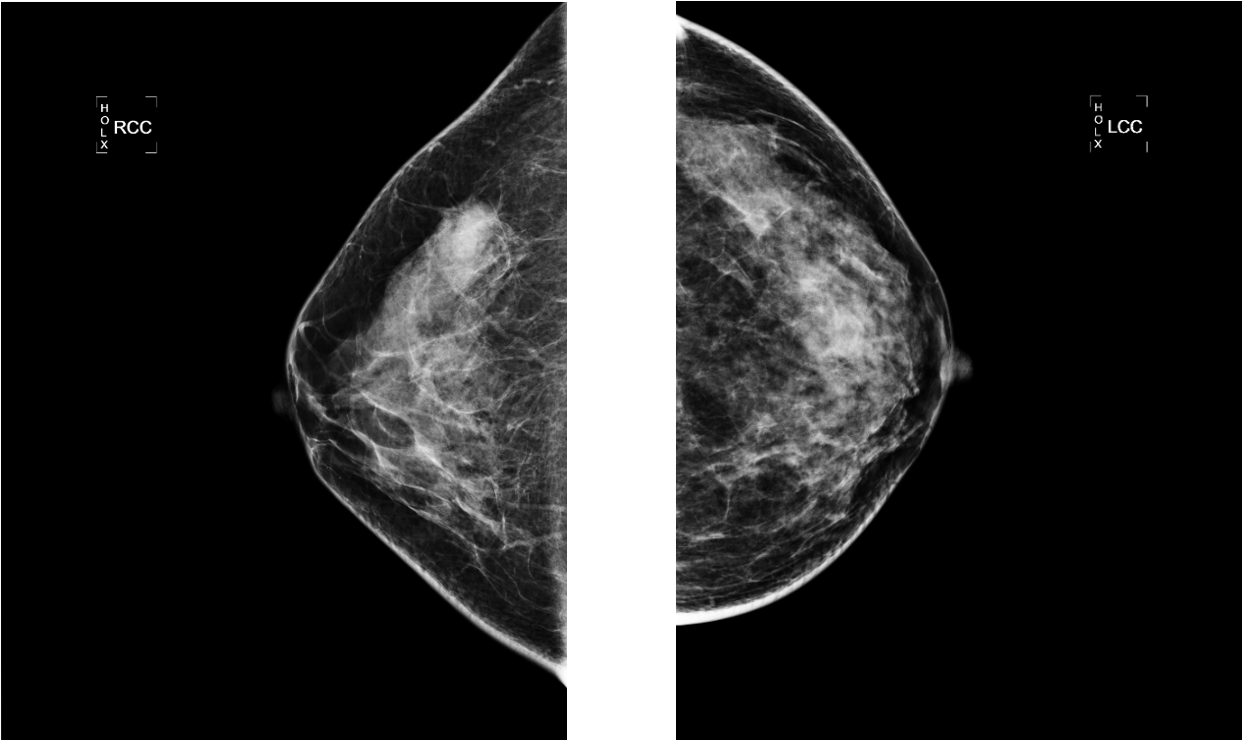
\includegraphics[width=1.0\textwidth]{intro_data}
    \bicaption{良恶性乳腺钼靶数据对比}{The malignant and benign mammography}
    \label{fig:intro_data}
	\end{figure}
	\item 医院有自己的标准,比如医生更关注敏感度和特异度,而不怎么关注准确率等传统计算机视觉的评判标准。在医学领域,存在着样本类别极度不均衡等问题,也更需要对此进行设计符合医生实际情况的评判标准。标准制定的有效与否,决定了模型的好坏。
\end{itemize}

	医生的诊断常常会因为人为的误判而导致较高的误诊率,而且乳腺钼靶的分析需要丰富的临床经验,这对于医生要求更高。正因为基于乳腺钼靶诊断同时存在如上诸多难点,如果可以通过训练有足够区分能力的乳腺钼靶分类识别模型,就可以充分降低医生在寻找乳腺钼靶病灶的时间,而且一定程度上降低人为的误诊率,从而达到辅助医生进行诊断的效果,这也充分验证了基于深度学习的乳腺钼靶的分类算法研究的必要性和重大意义。


\section{研究现状}
\subsection{乳腺影像学计算机辅助诊断方法}
随着计算机技术和统计机器学习算法的发展,CAD在医学影像领域获得了快速发展。CAD技术理论上可以应用于多种影像技术,通常医学影像学中计算机辅助诊断分为三步。

图像的处理过程(预处理),其目的是把病变从正常结构中提取出来。在这里图像处理的目的是使计算机易于识别可能存在的病变,让计算机能够从复杂的解剖背景中将病变及可疑结构识别出来。通常此过程先将图像数字化(经过一定的AD转换),一般用扫描仪将图像扫描,如果原始图像已经为数字化图像,如DR、CT、MRI图像则可省去此步。针对不同的病变,需要采用不同的图像处理和计算方法,基本原则是可以较好地实现图像增强和图像过滤,并通过上述设计好的处理过程,计算机得以将可疑病变从正常解剖背景中分离、显示出来。

图像征象的提取(特征提取)或图像特征的量化过程。目的是将第一步提取的病变特征进一步量化,即病变的征象分析量化过程。所分析征象是指对病变诊断具有价值的影像学表现,如病变的大小、密度、形态特征等。
数据处理过程。将第二步获得的图像征象的数据资料输入人工神经元网络等各种数学或统计算法中,形成CAD诊断系统,运用诊断系统,可以对病变进行分类处理,进而区分各种病变,即实现疾病的诊断。

而基于深度学习的CAD系统的算法大体上可分成四类:基于受限玻尔兹曼机(RBM)的模型,卷积神经网络(CNN),基于自编码(autoencoder)的模型,以及基于稀疏编码的模型(见\ref{tab:cad})\cite{4陈诗慧2017基于深度学习和医学图像的癌症计算机辅助诊断研究进展}

\newcommand{\tabincell}[2]{\begin{tabular}{@{}#1@{}}#2\end{tabular}}
\begin{table}[!htbp]
    \bicaption{基于深度学习的CAD系统算法\cite{4陈诗慧2017基于深度学习和医学图像的癌症计算机辅助诊断研究进展}}{CAD system algorithm based on deep learning\cite{4陈诗慧2017基于深度学习和医学图像的癌症计算机辅助诊断研究进展}}
    \label{tab:cad}
    \centering
    \footnotesize% fontsize
    \setlength{\tabcolsep}{4pt}% column separation
    \renewcommand{\arraystretch}{1.2}%row space 
    \begin{tabular}{ccc}
        \hline
         基于深度学习的算法 & \multicolumn{2}{c}{算法名称} \\
        \hline
         基于CNN的方法& \multicolumn{2}{c}{Alexnet,Clarifai,SPP,VGG,GoogleNet} \\
         基于RBM的方法& \multicolumn{2}{c}{\tabincell{c}{深信度网络(deep belief networks, DBN),\\
        深度玻尔兹曼机(deep Boltzmann machine, DBM), \\
        深度能量模型(deep energy model, DEM)}} \\
		基于自编码的方法& \multicolumn{2}{c}{\tabincell{c}{稀疏自编码器(sparse autoencoder, SAE),\\	
去噪自编码器(denoising autoencoder, DAE), \\
收缩自编码器(contractive autoencoder, CAE)}} \\
        基于稀疏编码的方法& \multicolumn{2}{c}{\tabincell{c}{稀疏编码空间金字塔配对,\\
        	拉普拉斯稀疏编码,\\局部坐标编码,\\超向量编码}} \\
        \hline
    \end{tabular}
\end{table}
尽管乳腺钼靶影像目前被认为是早期检查乳腺癌最可靠的方式,能够减少18\%-30\%的致死率,但其对比度不高,肿瘤与周围正常组织的分界不明显,这会导致10\%-30\%的癌症漏检。由于这个原因,在最近几十年,相关的和乳腺钼靶结合共同诊断分析的技术不断提出来\cite{郑光远2018医学影像计算机辅助检测与诊断系统综述},主要包括以下几种:
\begin{itemize}
	\item 基于乳腺超声图像的CAD系统	
	
	作为乳腺X光影像乳腺病变检查的技术辅助,引入了超声波检查,主要对影像学上致密的乳房提供更精确的评估。当这两种技术结合使用时,鉴别囊性结节和实性结节可减少了 25\%-35\%的活检数量,大大提高了有效率。
	\item 基于CT图像的乳腺癌症CAD系统
	
	由于乳腺钼靶摄影对病变的显示存在非显著性和误报问题,这会导致不必要的阴性穿刺活检。锥束乳腺CT扫描仪(bCT)作为一种新的专用影像方法,能够生成高质量的层析数据以提高乳腺组织和结构的可视化,并使病灶显示更显著。
	
	\item 基于MRI图像的乳腺癌症CAD系统
	
	 20世纪90年代以来,乳腺MRI就开始被用于表征和检测乳腺病变。MRI的敏感度非常高,可达到 78\%-98\%,但其特异度不足,只有 43\%-75\%。近些年发展起来的计算机辅助诊断软件的目的主要是为了使 MRI 分析
和报告更加便利,或试图进一步突出显示检测到的病变。
\end{itemize}

综合CAD的发展,现有的乳腺钼靶的CAD系统只能标出可能的区域,但并不能提供诊断和分型,对于中国女性致密性乳腺的特点也很难刻画病灶位置以辅助医生进行诊断,漏诊,误诊的现象时有发生,所以并不能有效地减少工作量。大多数的CAD耗时比较长,常规临床应用存在很大的难度。然而医疗影像的识别分析工作,对于人工智能的需求已然越来越强烈。目前我国医学影像数据的年增长率约为30\%,而放射科医师数量的年增长率约为4.1\%,放射科医师的数量增长远不及影像数据的增长,这意味着放射科医师在未来处理影像数据的压力会越来越大,甚至远远超过负荷。
\subsection{深度学习技术的发展}
随着谷歌的AlphaGo战胜韩国棋手李世石之后,深度学习从学术界的热点技术,变为大众热捧的热门技术,成为当前人工智能热潮中,最吸引眼球的技术方向。深度学习也从传统的图像、视频、语音识别领域,向文本处理、自然语言理解、人机对话、情感计算等各方面渗透。

深度学习理念,在上世纪六七十年代就有人提出过,但是由于缺乏有效的算法,没有形成规模应用。在上世纪80年代,由于出现了BP算法\cite{5riedmiller1993direct},多层前馈网络也曾经风靡一时,但是由于误差反向传播(BP)算法,对权值的调整从输出层开始,效果会每层递减,因此训练多层网络速度会变慢,而且多层网络额外增加了很多参数,需要更多的训练样本,由于当时计算能力的限制,最终多层前馈网络也没有流行起来。

随着技术的方法和计算能力的增强,以前制约深度学习的条件逐渐得到了解决,尤其是人们意识到,以前的神经网络,需要研究人员对问题进行深入的研究,提取出问题的关键属性,然后才是设计合适的神经网络,然后训练神经网络来解决这个问题。人们发现,在整个过程中,最困难的地方并非神经网络本身,而是抽取所研究问题的特征,这才是制约神经网络应用的核心问题。基于对这个问题的认识,逐渐出现了利用非监督学习网络来获取所研究问题的特征,然后再采用监督学习方式来训练网络,不仅可以使最为费时费力的特征提取来自动化,而且还可以对网络进行预训练,降低网络训练工作量以及所需训练样本。正是因为上述原因,深度学习技术才会在十年前逐渐流行起来。

2006年,神经网络领域的大师Geoffrey Hinton教授与其博士生在《Science》和相关期刊上发表了论文,首次提出了“深度置信网络(DBN)\cite{6hinton2006fast}”的概念。与传统的训练方式不同,“深度置信网络”有一个“预训练”(pre-training)的过程,这可以方便的让神经网络中的权值找到一个接近最优解的值,之后再使用“微调”(fine-tuning)技术来对整个网络进行优化训练。这两个技术的运用大幅度减少了训练多层神经网络的时间。他给多层神经网络相关的学习方法赋予了一个新名词——“深度学习”。

2012年,Hinton教授的研究团队参加了斯坦福大学李飞飞教授等组织的ImageNetILSVRC大规模图像识别评测任务\cite{7krizhevsky2012imagenet}。该任务包括120万张高分辨率图片,1000个类比。Hinton教授团队使用了全新的多层CNN(卷积神经网络,Convolutional Neural Networks,简称CNN)结构,突破性地将图像识别错误率从26.2\%降低到了15.3\%。这一革命性的技术,让神经网络深度学习以极快的速度跃入了医疗和工业领域,这才有了后来一系列使用该技术的医学影像公司的出现。深度学习在计算机视觉方面取得的突破性进展是其应用在医疗影像上的主要因素,微软亚洲研究院于2015年开发的ResNet\cite{8he2016deep}模型在ImageNet自然图片数据集上的识别准确率超过了人类,为丰富多彩的视觉应用提供了很好的基础模块。

深度学习在医疗领域最激动人心的应用,无疑是在在医学诊断方面的应用。谷歌的DeepMind和IBM的watson,都在这方面积极布局,尤其是watson,在某些特定领域,其诊断精度已经超过了人类专家。由于医疗中病例大多数为非结构化文本数据,因此采用多层限制性波尔兹曼机(RBM)\cite{9nair2010rectified}堆叠成的深度信念网络(DBN),可以自动提取文本病例中的特征,可以有效的学习病历中的知识,同时可以高效地进行诊断。2016年至2018年,《Nature》等顶级学术期刊也将目光投向了基于医学影像的深度学习应用,包括糖尿病视网膜病变诊断\cite{10morris2017technology},儿童白内障分类诊断\cite{11long2017artificial}和皮肤癌病变诊断\cite{12esteva2017dermatologist}等等,这些成果表明计算机经过训练甚至可以超过资深专家的诊断准确率,预示了其在计算机辅助诊断方面巨大的应用潜力。2018年,Cell杂志上同时报道了基于深度学习的视网膜疾病诊断工具\cite{13kermany2018identifying},证明了AI系统在图像诊断方面具有普遍适用性。

目前在乳腺癌问题上,最为成熟的是病理活检方面,如去年发布在《Nature》封面上的一篇关于乳腺癌病理的自动检测模型\cite{14liu2017detecting},自动检测的准确率首次超过临床医生,达到了93\%-95\%。除此外,还包括核磁前列腺癌区域的自动检测、脑部肿瘤的识别和分割,还有应用非常普遍和广泛的乳腺钼靶的钙化点的自动检测,以及胸片的自动检测,所有的方法都依赖于大量的数据以及有效的数据标注,并利用卷积神经网络,递归神经网络等深度神经网络结构自动获取特征表达能力,去掉繁杂的人工特征工程,进行病灶的定性自动检测。

我们有理由相信深度学习同样能在乳腺影像学诊断方面大放光彩,有望加速有关可治疗性疾病的诊断,从而促进疾病的早治疗,最终改善病人的临床结果,取得成功。
\subsection{深度学习在乳腺乳腺上的发展}
采用CNN,可以极大提高识别率,同时降低对原始图片质量的要求,同时可以降低对训练样本数量的要求,因此CNN在医学影像处理方面,应该是目前应用最广泛也是最成功的领域。

目前主流的方法是直接对乳腺钼靶进行整图分类,应用迁移学习\cite{15pan2010survey}或者切割出病灶位置进行检测的方式使得结果更加鲁棒。比如MICCAI2017收录的\cite{16zhu2017deep}提出的模型的总体框架是,首先对输入图像进行分割、缩放得到感兴趣的区域,通过CNN提取很多区块后,用线性回归分类器得到可能性排序,最后根据机器学习模型得到影像的判定结果输出, 其在INBREAST\cite{27moreira2012inbreast}乳腺钼靶公开数据集上达到ACC为0.90,AUC为0.8586的结果。LÉVY D等\cite{17levy2016breast}以及SHEN L.等\cite{18shen2017end}论文中
使用从传统自然数据学习到的AlexNet\cite{19krizhevsky2012imagenet},VGG\cite{20simonyan2014very}等模型迁移到公开的乳腺钼靶数据集DDSM\cite{21lee2018curated, 22lee2017curated,23clark2013cancer}进行验证测试,通过使用热图,移动窗口等方式获取候选框,进而对病灶位置进行切割形成patch,之后对病灶位置使用数据增广方式,最后SHEN L.等\cite{18shen2017end}在测试集上最好的结果ACC为0.90。

除了在使用迁移学习以及切割出病灶位置的思路外,已有的基于深度学习的乳腺钼靶分类算法也考虑到乳腺钼靶的数据特点,进而通过融合不同分类模型、不同分辨率、多个角度乳腺钼靶图片来提高模型的性能。比如 DHUNGEL N等\cite{24dhungel2017fully}使用multi-model的思路,先训练多个分类模型来对单一乳腺钼靶图片进行学习,最后融合每个模型结果达到较好的结果。CARNEIRO N D G等\cite{25carneiroautomated}则使用了multi-scale,由于乳腺钼靶图片较大,可以先将同一张乳腺钼靶图片缩放到不同尺度,之后融合多个不同分辨率的乳腺钼靶图片来增强对单一乳腺钼靶图片的学习能力。而GERAS K J等\cite{26geras2017high}则考虑同一病人下的乳房拥有多个不同角度(MLO和CC),通过利用multi-direction的思想,结合两个不同角度的乳腺钼靶学习结果,来加强对单一乳房的识别效果。工业界对该问题也是特别关注,比如Google的DeepMind和腾讯觅影计划在内的工业界目前所采用的方法也是对整图进行分类,其中腾讯觅影计划对肿块检测的良恶性判别的敏感度达到0.90,特异度达到0.96。

上述模型均只是考虑到直接使用整图信息进行分类,之后在此基础上使用各种multi思路来综合考虑并加强分类的结果。这些模型并没有充分利用到乳腺病灶的信息,而且,所采用的数据来自公开的数据集,常见的是INBREAST\cite{27moreira2012inbreast}和DDSM\cite{21lee2018curated, 22lee2017curated,23clark2013cancer}。这些数据集所采用的数据均来自西方女性,并不完全适用于东方女性特有的致密性乳腺。

少数的几种从检测角度对乳腺钼靶进行检测分类的,比如从这一角度考虑的论文\cite{28ribli2018detecting, al2017detection, 29ribli2018detecting}所采用的方法,都是在带有恶性乳腺肿瘤标注信息上的数据集上使用主流的FasterR-CNN\cite{30ren2015faster}或YOLO\cite{32redmon2016you}模型进行检测。虽然充分利用到了检测信息,但是忽略了大部分的没有带有标注信息的正常数据(包括疑似恶性肿瘤的良性和阴性数据),造成了数据资源的浪费,而且由于没有充分考虑到恶性和正常数据分布的各异性,使得结果容易偏向恶性数据,造成该训练下的检测模型在对正常数据进行检测时,会造成很大的假阳性率。

\subsection{存在的问题及解决方案}
目前的基于深度学习的乳腺钼靶分类算法大多考虑到迁移学习方法。从目前的研究现状可以知道,分类角度主要采用切割patch方式提取出病灶信息进而进一步考虑和使用多模型,多角度融合等multi思路提升模型效果,这么做对于本文而言,一方面加大了复杂度,而且未充分利用数据自带的检测信息;检测角度则更多的问题在于只考虑到有标注信息的数据,对于实际应用场景,尤其对于医疗领域的影像数据而言,常常存在没法标注的数据,这就使得现有的模型无法解决这问题,并且需要在数据的基础上创新性的设计全新模块。

针对上述问题,本论文期望从天津肿瘤医院获取到的真实数据出发,在基于现有深度学习模型基础上,对数据进行尝试性的研究工作后,提出全新的适用于本数据的模块与方法,从而同时满足性能与效率的要求。

\section{主要研究内容}
由于东方女性偏致密性乳腺,属于致密性乳腺分型,而肿块是众多乳腺癌表现中最为常见的。针对于前面介绍的研究对象乳腺钼靶及其发展现状等,毕设工作将完成基于深度学习的乳腺钼靶分类算法的研究工作,主要研究内容是:
针对医院提供的特有的东方女性肿块型致密性乳腺钼靶病例,也就是带有标注的恶性乳腺钼靶和正常乳腺钼靶病例(没有标注的良性和阴性乳腺钼靶病例),基于深度学习等技术,以恶性乳腺钼靶病例图片数据为重点研究对象,并辅以正常乳腺钼靶病例图片数据,使得设计的分类检测模型可以分类出恶性及正常乳腺钼靶病例,且识别恶性乳腺钼靶图片数据中病灶位置。

从本质上而言,本文所要学习的标注信息数据并不全面,所以在具体模型设计时应当充分考虑这一点,并针对模型结果进行相应的损失函数设计以充分利用恶性样本标注信息及未标注的正常样本信息。
具体而言包括以下部分:
\subsection{需求分析,确定评判标准}
明确数据采集格式要求,分析医学数据,进行去除噪声数据等操作;根据天津肿瘤医院的实际要求及计算机视觉的知识,设定评判标准。
\subsection{实现基于深度学习的乳腺钼靶分类模型}
调查已有的方法及模型,对比分析优劣;使用原始的Faster R-CNN,根据数据特点,分阶段训练乳腺钼靶数据并得到分类检测结果。
\subsection{设计全新损失函数,改进并设计全新分类检测模型}
根据数据特点及实现现象,对实验结果进行优劣分析,引入全新损失函数,改进原始Faster R-CNN模型。
\subsection{编程实现,完成不同模型之间的对比分析}
基于评判标准及设计的深度学习模型,完成源码的实现,并借助于实验结果对模型模块进行更新与对比分析,从而为基于深度学习的乳腺钼靶及医学影像的算法研究提供新思路。
\section{本文结构及内容提要}
论文的第一章部分主要介绍了乳腺癌及乳腺钼靶的相关医学知识及诊断方法,以及目前所采用的基于深度学习乳腺钼靶的分类检测思路,对于其中的优劣势分别进行了讨论和考虑,并重点介绍了基于深度学习的乳腺钼靶分类算法的研究的必要性与重要性,对于之后的工作进行了整体的思路设计。

论文的第二章详细介绍了本文所使用到的深度学习技术,包括卷积神经网络,基于卷积神经网络技术基础发展的物体检测模型,为解决数据量少而使用的迁移学习,为了学习恶性及正常样本之间区别而引入的度量学习,在设计标准中根据实际情况而使用的弱监督学习等。

论文的第三章具体介绍了医学数据,尤其乳腺钼靶数据的特点,根据数据特点进行了数据预处理,划分以及标准制定,为后期模型的设计与评判提供依据。

论文的第四章主要介绍了从两阶段角度考虑下模型的设计及结果。由于恶性及正常数据之间存在明显的区别,所以在本章中先是考虑对恶性数据进行模型学习,再学习恶性及正常数据之间微弱的区别,通过调参达到一定的效果后,对结果进行分析,从而引出后续的第四章的一阶段模型的设计及研究。

第五章是在第四章已经研究的基础上,试图从降低复杂度的角度考虑提高模型的运行速度,并基于对数据特点的分析上,对RPN网络设计top likelihood loss损失函数,并对数据之间微弱区别引入similarity loss全新损失函数。在保证和两阶段差不多的诊断性能下,提升模型运行的效率。

第六章总结了本文的研究内容,并提出了当前研究方法的不足和未来本领域面临的挑战。

